% !TEX root = ../main.tex
\chapter{Contexto y estado de la técnica}

Este capítulo presenta los fundamentos conceptuales y el estado actual de la técnica en computación cuántica aplicada a la ciencia de datos. Se revisan los trabajos previos más relevantes, se identifican las limitaciones de los enfoques existentes y se sitúa la contribución de este trabajo en el contexto académico y profesional actual.

\section{Antecedentes históricos}

El origen formal de la computación cuántica como disciplina se remonta a los trabajos de \cite{feynman1982}, quien propuso el uso de sistemas cuánticos para simular la naturaleza de forma eficiente, argumentando que un computador clásico no podía simular un sistema cuántico sin un coste exponencial. Poco después, \cite{deutsch1985} formalizó el concepto de computador cuántico universal y demostró la existencia de problemas que un computador cuántico podría resolver de forma más eficiente que cualquier computador clásico.

El interés por la computación cuántica se intensificó con los algoritmos de \cite{shor1994} y \cite{grover1996}, que demostraron aceleraciones exponenciales y cuadráticas respectivamente frente a los mejores algoritmos clásicos conocidos para factorización de enteros y búsqueda no estructurada. Estos resultados establecieron la viabilidad teórica de la ventaja cuántica y sentaron las bases para el desarrollo de hardware cuántico experimental. Los fundamentos formales del modelo de computación cuántica, incluyendo los postulados de la mecánica cuántica, las puertas cuánticas y los circuitos cuánticos, se encuentran desarrollados en detalle en \cite{nielsen2010}.

En paralelo, el campo del aprendizaje automático experimentó un crecimiento extraordinario impulsado por el aumento de la capacidad computacional y la disponibilidad de grandes volúmenes de datos \citep{jordan2015}. La confluencia de ambas disciplinas dio lugar al campo del aprendizaje automático cuántico (\textit{Quantum Machine Learning}, QML), cuyo objetivo es explorar si las capacidades de procesamiento cuántico pueden ofrecer ventajas en tareas de aprendizaje estadístico \citep{biamonte2017}.

\section{Computación cuántica en la era NISQ}

El estado actual del hardware cuántico se enmarca en lo que \cite{preskill2018} denominó la era NISQ (\textit{Noisy Intermediate-Scale Quantum}), caracterizada por dispositivos con entre 50 y varios cientos de qubits físicos, afectados por errores de decoherencia y ruido cuántico, y sin capacidad para implementar corrección de errores cuánticos a gran escala. Esta realidad impone restricciones fundamentales sobre la profundidad de los circuitos ejecutables y la fiabilidad de los resultados obtenidos.

\begin{figure}[!htbp]
\centering
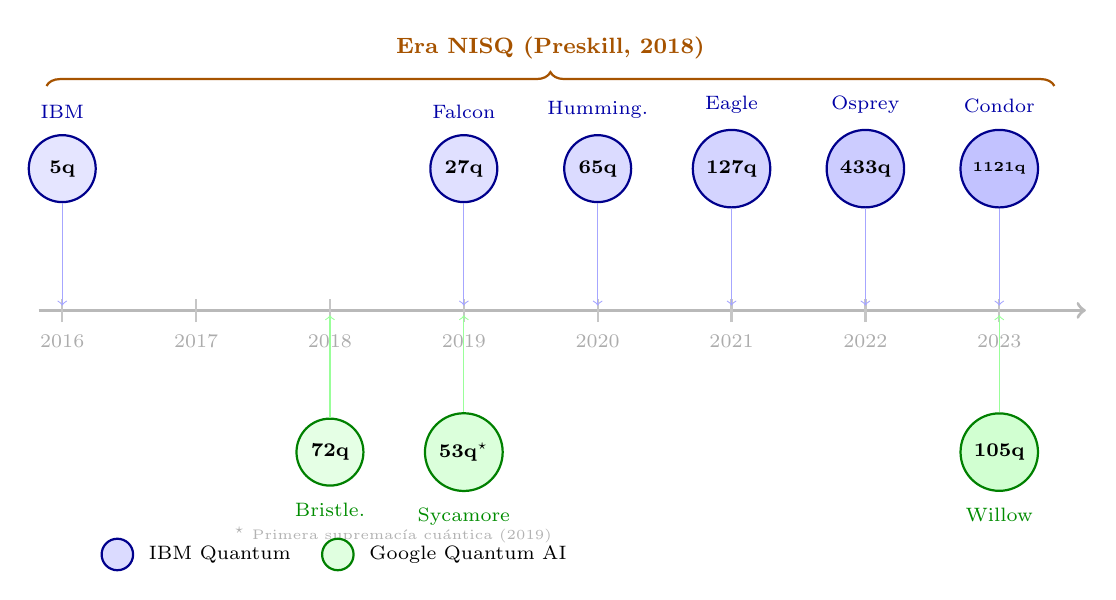
\begin{tikzpicture}[font=\scriptsize, thick]
  % Eje temporal
  \draw[->, very thick, gray!55] (-0.3, 0) -- (13.0, 0);

  % Marcas y etiquetas de año
  \foreach \yr/\x in {2016/0, 2017/1.7, 2018/3.4, 2019/5.1, 2020/6.8, 2021/8.5, 2022/10.2, 2023/11.9} {
    \draw[gray!45] (\x, -0.15) -- (\x, 0.15);
    \node[below=5pt, gray!65] at (\x, 0) {\yr};
  }

  % ── IBM (arriba) ──────────────────────────────────────────────────────────
  \node[circle, draw=blue!55!black, fill=blue!10, minimum size=0.85cm, align=center,
        font=\bfseries\scriptsize] (i1) at (0, 1.8) {5q};
  \node[above=2pt, blue!65!black, align=center, font=\scriptsize] at (i1.north) {IBM};
  \draw[->, blue!35, thin] (i1.south) -- (0, 0.06);

  \node[circle, draw=blue!55!black, fill=blue!12, minimum size=0.85cm, align=center,
        font=\bfseries\scriptsize] (i2) at (5.1, 1.8) {27q};
  \node[above=2pt, blue!65!black, align=center, font=\scriptsize] at (i2.north) {Falcon};
  \draw[->, blue!35, thin] (i2.south) -- (5.1, 0.06);

  \node[circle, draw=blue!55!black, fill=blue!14, minimum size=0.85cm, align=center,
        font=\bfseries\scriptsize] (i3) at (6.8, 1.8) {65q};
  \node[above=2pt, blue!65!black, align=center, font=\scriptsize] at (i3.north) {Humming.};
  \draw[->, blue!35, thin] (i3.south) -- (6.8, 0.06);

  \node[circle, draw=blue!55!black, fill=blue!17, minimum size=0.85cm, align=center,
        font=\bfseries\scriptsize] (i4) at (8.5, 1.8) {127q};
  \node[above=2pt, blue!65!black, align=center, font=\scriptsize] at (i4.north) {Eagle};
  \draw[->, blue!35, thin] (i4.south) -- (8.5, 0.06);

  \node[circle, draw=blue!55!black, fill=blue!20, minimum size=0.85cm, align=center,
        font=\bfseries\scriptsize] (i5) at (10.2, 1.8) {433q};
  \node[above=2pt, blue!65!black, align=center, font=\scriptsize] at (i5.north) {Osprey};
  \draw[->, blue!35, thin] (i5.south) -- (10.2, 0.06);

  \node[circle, draw=blue!55!black, fill=blue!24, minimum size=0.85cm, align=center,
        font=\bfseries\tiny] (i6) at (11.9, 1.8) {1121q};
  \node[above=2pt, blue!65!black, align=center, font=\scriptsize] at (i6.north) {Condor};
  \draw[->, blue!35, thin] (i6.south) -- (11.9, 0.06);

  % ── Google (abajo) ────────────────────────────────────────────────────────
  \node[circle, draw=green!50!black, fill=green!10, minimum size=0.85cm, align=center,
        font=\bfseries\scriptsize] (g1) at (3.4, -1.8) {72q};
  \node[below=2pt, green!55!black, align=center, font=\scriptsize] at (g1.south) {Bristle.};
  \draw[->, green!40, thin] (g1.north) -- (3.4, -0.06);

  \node[circle, draw=green!50!black, fill=green!14, minimum size=0.85cm, align=center,
        font=\bfseries\scriptsize] (g2) at (5.1, -1.8) {53q$^{\star}$};
  \node[below=2pt, green!55!black, align=center, font=\scriptsize] at (g2.south) {Sycamore};
  \draw[->, green!40, thin] (g2.north) -- (5.1, -0.06);

  \node[circle, draw=green!50!black, fill=green!18, minimum size=0.85cm, align=center,
        font=\bfseries\scriptsize] (g3) at (11.9, -1.8) {105q};
  \node[below=2pt, green!55!black, align=center, font=\scriptsize] at (g3.south) {Willow};
  \draw[->, green!40, thin] (g3.north) -- (11.9, -0.06);

  % Nota supremacía
  \node[font=\tiny, gray!60, align=left] at (4.2, -2.85)
    {$^{\star}$ Primera supremacía cuántica (2019)};

  % Llave "Era NISQ"
  \draw[decorate, decoration={brace, amplitude=5pt}, thick, orange!65!black]
    (-0.2, 2.85) -- (12.6, 2.85);
  \node[above=6pt, orange!65!black, font=\footnotesize\bfseries] at (6.2, 2.85)
    {Era NISQ (Preskill, 2018)};

  % Leyenda
  \node[circle, draw=blue!55!black, fill=blue!14, minimum size=0.4cm] at (0.7, -3.1) {};
  \node[right=2pt, font=\scriptsize] at (0.9, -3.1) {IBM Quantum};
  \node[circle, draw=green!50!black, fill=green!12, minimum size=0.4cm] at (3.5, -3.1) {};
  \node[right=2pt, font=\scriptsize] at (3.7, -3.1) {Google Quantum AI};
\end{tikzpicture}
\caption{Evolución del hardware cuántico en la era NISQ (2016--2023). Los nodos superiores (azul) corresponden a procesadores IBM Quantum; los inferiores (verde) a Google. Los números indican el recuento de qubits físicos disponibles. La supremacía cuántica de Google Sycamore (2019) marcó el primer experimento que superó la simulación clásica exacta para una tarea específica.}
\label{fig:timeline_hardware}
\end{figure}

En respuesta a estas limitaciones, se han desarrollado los algoritmos variacionales cuánticos (\textit{Variational Quantum Algorithms}, VQA), que combinan un circuito cuántico parametrizado con un optimizador clásico en un bucle híbrido \citep{cerezo2021}. Entre los más destacados se encuentran el Quantum Approximate Optimization Algorithm (QAOA) \citep{farhi2014}, diseñado para problemas de optimización combinatoria, y el Variational Quantum Eigensolver (VQE) \citep{peruzzo2014}, orientado a la simulación de sistemas moleculares. Estos algoritmos son actualmente los candidatos más prometedores para demostrar ventaja cuántica práctica en hardware NISQ.

No obstante, la comunidad científica mantiene un debate activo sobre si los algoritmos NISQ pueden alcanzar ventaja cuántica genuina frente a los mejores algoritmos clásicos. \cite{cerezo2023} analizan en profundidad el fenómeno de los \textit{barren plateaus}, gradientes exponencialmente pequeños que dificultan el entrenamiento de los circuitos variacionales a medida que el número de qubits crece, comprometiendo la escalabilidad de estos enfoques.

\section{Aprendizaje automático cuántico}

El aprendizaje automático cuántico ha sido objeto de una revisión sistemática exhaustiva por parte de \cite{biamonte2017}, quienes identificaron cuatro categorías principales de algoritmos QML según la naturaleza del procesador (clásico o cuántico) y de los datos (clásicos o cuánticos). Para el contexto de este trabajo, el caso más relevante es el de datos clásicos procesados mediante algoritmos cuánticos (CC$\rightarrow$CQ en la nomenclatura de los autores).

Los métodos basados en kernels cuánticos (\textit{Quantum Kernel Methods}) han recibido especial atención. \cite{schuld2021} demostraron que los circuitos cuánticos pueden actuar como mapas de características (\textit{feature maps}) hacia espacios de Hilbert de alta dimensión, y que la estimación del kernel inducido puede ser computacionalmente difícil de simular clásicamente bajo ciertas condiciones. Sin embargo, \cite{huang2021} establecieron condiciones teóricas precisas bajo las cuales los kernels cuánticos pueden ofrecer una ventaja de aprendizaje sobre los kernels clásicos, concluyendo que dicha ventaja depende críticamente de la estructura geométrica de los datos de entrada.

En el contexto de la clasificación supervisada con datos reales, \cite{haug2023} propusieron el uso de medidas aleatorizadas para escalar los métodos de kernel cuántico a conjuntos de datos de gran tamaño, abordando uno de los principales cuellos de botella prácticos de estos métodos. Los resultados experimentales mostraron rendimientos competitivos frente a kernels clásicos en benchmarks estándar, aunque con una ventaja aún limitada.

\section{Optimización cuántica aplicada}

El QAOA, propuesto originalmente por \cite{farhi2014}, es un algoritmo híbrido cuántico-clásico que aproxima la solución de problemas de optimización combinatoria formulados como problemas de satisfacibilidad cuadráticas binarias (QUBO). Su aplicabilidad se extiende a problemas de relevancia empresarial como la optimización de rutas \citep{lucas2014}, la asignación de recursos, la segmentación de mercado y la optimización de carteras financieras.

\cite{zhou2020} estudiaron el rendimiento del QAOA en función de la profundidad del circuito ($p$) y demostraron que, para problemas de tamaño moderado, la calidad de la aproximación mejora monotónamente con $p$. No obstante, la ventaja cuántica del QAOA frente a los mejores algoritmos clásicos heurísticos sigue siendo una cuestión abierta para instancias de gran escala \citep{farhi2014}.

Desde una perspectiva aplicada, \cite{vikstaal2020} evaluaron la aplicabilidad del QAOA a problemas de optimización financiera reales, identificando los principales desafíos prácticos: la necesidad de un gran número de shots para estimar expectativas con precisión suficiente, la sensibilidad a los parámetros iniciales y la degradación del rendimiento en hardware ruidoso. Estos resultados subrayan la importancia de realizar evaluaciones experimentales sobre datos reales más allá de las pruebas de concepto teóricas.

\section{Análisis crítico de los trabajos previos}

La revisión de la literatura permite identificar un conjunto de limitaciones recurrentes en los estudios existentes que este trabajo pretende abordar:

\begin{itemize}
    \item \textbf{Uso predominante de datos sintéticos o académicos}: la mayoría de los estudios comparativos utilizan conjuntos de datos de benchmarks estándar (Iris, MNIST, MaxCut), que no reflejan la complejidad y el ruido inherentes a los datos empresariales reales \citep{biamonte2017, haug2023}.

    \item \textbf{Ausencia de comparación sistemática con métodos clásicos consolidados}: muchos trabajos evalúan el rendimiento cuántico de forma aislada, sin contrastar con técnicas clásicas de referencia como SVM, Random Forests o algoritmos genéticos en las mismas condiciones experimentales \citep{fastovets2019}.

    \item \textbf{Foco en la viabilidad teórica más que en la aplicabilidad práctica}: los análisis de ventaja cuántica suelen estar formulados en términos asintóticos o bajo supuestos ideales de hardware, sin considerar las restricciones reales de los dispositivos NISQ actuales \citep{cerezo2023}.

    \item \textbf{Escasa consideración de la integración en pipelines productivos}: los trabajos existentes raramente abordan la cuestión de cómo los módulos cuánticos podrían integrarse en arquitecturas de análisis de datos clásicas ya existentes en entornos empresariales \citep{cerezo2021}.
\end{itemize}

Este trabajo contribuye a superar estas limitaciones mediante un diseño experimental que combina datos reales de negocio, comparación directa con métodos clásicos de referencia y una evaluación orientada a la viabilidad de integración práctica.